\documentclass{article}

\usepackage[T1]{fontenc}    %Schriftart des Dokumentes
\usepackage[ngerman]{babel} %Dokumentensprache, hier Deutsch
\usepackage{amsmath, amssymb, stmaryrd} %mathematische Schriftzeichen
\usepackage{graphicx} %Einfügen von Grafiken
\usepackage{wrapfig}
\usepackage{bm}
\usepackage{subfig}
\usepackage{newclude}
\usepackage{pdfpages}

\setlength{\parindent}{0pt} %Einrückung von Absätzen auf null gesetzt
\setlength{\parskip}{10pt} %Abstand zischen Absätzen auf 10pt gesetzt

\title{Versuch 234: Lichtwellen und Gitterspektroskopie}
\author{Matthias Kuntz}
\date{19.02.2024}

\renewcommand*\contentsname{Zusammenfassung}

\begin{document}

\maketitle

\tableofcontents

\newpage

%-------------------------EINLEITUNG-------------------------
\section{Einleitung}

Verschiedenste Körper strahlen auf verschiedenste Weisen Licht aus. Beginnend bei der Sonne am Himmel bis zu den Pixeln in unseren Displays gibt es vielfältige Ursprünge des Lichts. Noch interessanter wird es, wenn man untersucht welche Wellenlängen wie stark ausgestrahlt werden. Ziel dieses Versuches ist es, mehrere Lichtquellen und ihre abgestrahlten Spektren zu untersuchen und dabei die vielfältigen Unterschiede in Ursprung und Resultat aufzuzeigen. Hierzu wird die Gitterspektroskopie genutzt, eine Methode bei der ein sogenanntes Gitterspektrometer verwendet wird, um aufgenommenes Licht in seine Einzelteile aufzuspalten und digital zu untersuchen.  

\subsection{Physikalische Grundlagen}

\subsubsection{Temperaturstrahler}

Die erste Methode, wie ein Körper strahlen kann, ist als Temperaturstrahler. Jeder Körper, der eine Temperatur höher als 0K besitzt, strahlt elektromagnetische Strahlung aus. Ein ideales Modell ist hierbei der sogenannte "perfekte Schwarze Körper", ein solcher, der die auf ihn einfallende elektromagnetische Strahlung komplett absorbiert und somit nur eine Strahlung abhängig von der eigenen Temperatur abgibt. Ein solcher Körper besitzt somit ein maximales Emissionsvermögen mit $\epsilon = 1$. Die Intensitätsverteilung eines Schwarzen Körpers wird durch das Planck'sche Strahlungsgesetzt beschrieben:

\begin{equation}
    M_{\lambda}(\lambda, T) \ \text{d}A \ \text{d}\lambda = \frac{2 \pi h c^2}{\lambda^5} \frac{1}{\exp{\frac{hc}{\lambda k_B T}}-1} \ \text{d}A \ \text{d}\lambda
    \label{eq:planck}
\end{equation}

Hierbei steht $M_{\lambda}$ für die Strahlungsleistung, die vom Flächenelement d$A$ eines schwarzen Körpers mit homogener Temperatur $T$ im Wellenlängenbereich von $\lambda$ bis $\lambda + \text{d}\lambda$ ausgestrahlt wird. Das Maximum dieser Verteilung, ergo bei welcher Temperatur die Strahlungsleistung am größten ist, wird durch das Wien'sche Verschiebungsgesetz beschrieben:

\begin{equation}
    \lambda_{\text{max}} = \frac{1}{T} \ 2897,8 \mu \text{m} \cdot \text{K}
    \label{eq:wien}
\end{equation}

\begin{figure}[!h]
    \centering
    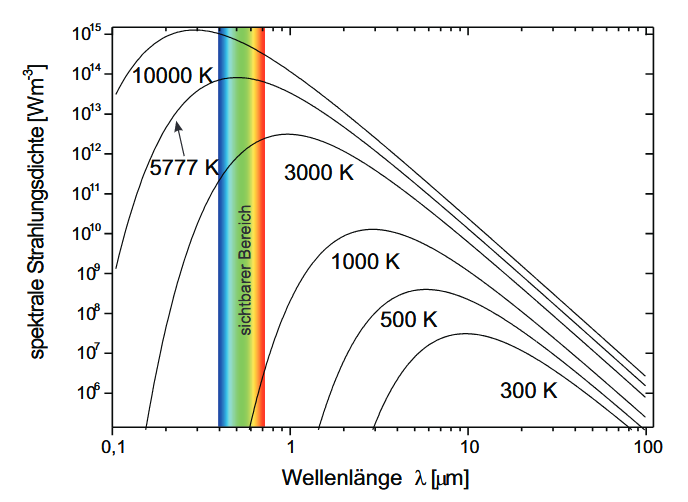
\includegraphics[width=0.9\textwidth]{graphics/bb.png}
    \caption{Strahlunsleistung eines Schwarzkörpers bei verschiedenen Temperaturen [Quelle: PAP2.1 Skript, S.113, 19.02.2024]}
    \label{fig:bbstrahlung}
\end{figure}

Eine häufige Charakterisierung von Licht erfolgt über die Farbtemperatur. Ein Körper mit 0K erscheint absolut schwarz. Bei steigenden Temperaturen wird nach und nach immer mehr farbiges Licht emittiert, beginnend bei rot und über grün, was sich mit dem rot zu einem orange bis gelblichen Ton vermischt. Bei etwa 5500K werden alle Wellenlängen des sichtbaren Lichts gleichstark emittiert und es erscheint weiß. Wird der Körper heißer wird mehr blau ausgesendet und er erscheint somit bläulicher. Umgangssprachlich wird Licht mit hohem Blauanteil Kaltlicht und solches mit hohem Rotanteil Warmlicht genannt.

Der schwarze Körper ist auch ein gutes Modell für die Sonne. Ihr Spektrum auf der Erde ist an sich kontinuierlich, allerdings durchzogen von Absorptionslinien, den sogenannten Fraunhoferlinien. Sie entstehen durch Absorption in der Sonnen- und Erdatmosphäre und zeigen somit charakteristische Verteilungen basierend auf der Zusammensetzung der beiden Atmosphären auf. Insbesondere die Absorptionslinien von Wasserdampf, Sauerstoff und Kohlendioxid sind sehr ausgeprägt. 

\begin{figure}[!h]
  \centering
  \subfloat[Fraunhoferlinien]{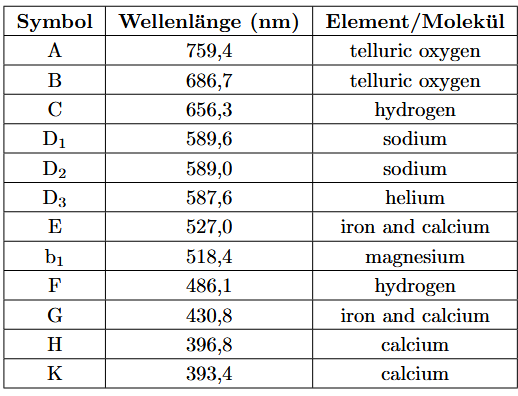
\includegraphics[width=0.5\textwidth]{graphics/fraunhoferlinien.png}\label{fig:fraunhoferlinien}}
  \hfill
  \subfloat[Balmer-Serie]{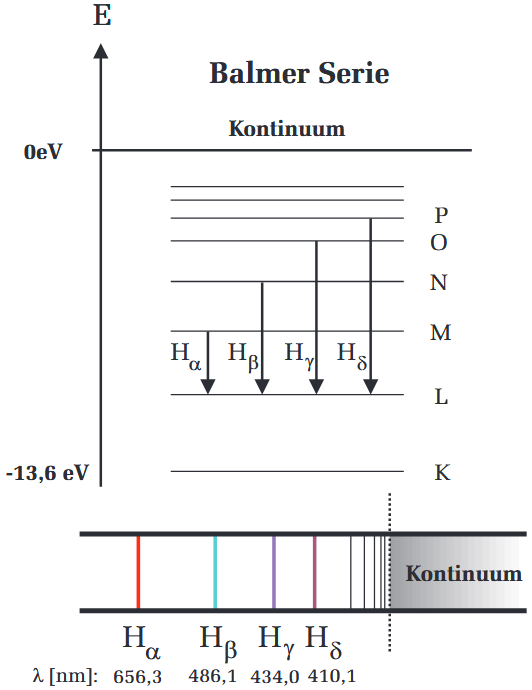
\includegraphics[height=5cm]{graphics/balmer.png}\label{fig:balmer}}
  \caption{Fraunhoferlinien und Balmer-Serie [Quelle: PAP2.1 Skript, S.125, 21.02.2024]}
  \label{fig:fraunh_balmer}
\end{figure}


\subsubsection{Nichttemperaturstrahler}

Im Gegensatz zu den Temperaturstrahlern senden Nichttemperaturstrahler nicht Wärmestrahlung aus, sondern stützen sich auf die Anregung bestimmter Atomzustände in Gasen oder Festkörpern oder die Rekombination von Elektron-Loch Paaren in Halbleitern. Sie haben nicht wie die Temperaturstrahler ein kontinuierliches, sondern ein diskretes Spektrum, das charakteristische Eigenschaften je nach verwendetem Material aufweist. Beispiele sind Leuchtstoffröhren, Leuchtdioden oder Laser. 

Da hierbei häufig viel UV-Strahlung abgegeben wird, werden Lampen meist mit einem fluoreszierenden Leuchtstoff beschichtet, der Fluoreszenslicht im sichtbaren Bereich ausstrahlt. 

\subsubsection{Absorption von Medien}

Läuft Licht auf seinem Weg durch ein Medium, wie beispielsweise durch eine Fensterscheibe, so wird ein Teil des Lichts vom Medium absorbiert. Quantitativ kann man die Absorption $A$ eines Mediums X aus der Intensität des Lichts ohne Medium $I_{\text{oX}}$ und der Intensität mit Medium $I_{\text{mX}}$ errechnen:

\begin{equation}
    A_{\text{X}} = 1 - \frac{I_{\text{mX}}}{I_{\text{oX}}}
    \label{eq:absorp}
\end{equation}

\subsubsection{Das Natriumspektrum} \label{DasNatriumspektrum}

Natrium bestitzt als alkaliatom ein wasserstoffartiges Spektrum. Durch das im Atom herrschende Potential wird die l-Entartung der Elektronen aufgehoben und die Energieniveas sind nun im allgemeinen nicht nur von der Hauptquantenzahl $n$, sondern auch von der Drehimpulsquantenzahl $l$ abhängig. In guter Näherung ergibt sich:

\begin{equation}
    E_{n, l} = -13,6 \text{eV} \ \frac{1}{(n - \Delta_{n,l})^2}
    \label{eq:Energ-Na}
\end{equation}

Hierbei hängt der Korrekturterm $\Delta_{n,l}$ nur geringfügig von $n$ ab und kann somit auch als $\Delta_{l}$ geschrieben werden. 

Somit gibt es verschiedene Übergänge mit verschiedenen Energiedifferenzen, die Licht mit unterschiedlichen Wellenlängen emittieren. Der Grundzustand eines Natrium-Valenzelektrons ist der 3s-Zustand. Es gibt nun drei Serien an Übergängen: Die Hauptserie mit Übergängen mp $\xrightarrow{}$ 3s, ergo zum Grundzustand, sowie die 1. und 2. Nebenserie mit den jeweiligen Übergängen md $\xrightarrow{}$ 3p und ms $\xrightarrow{}$ 3p. Am prägnantesten ist im Natriumspektrum das gelbe Dublett bei 589nm bestehend aus zwei Übergängen der Hauptserie. 

Welche Energieniveaus und welche Entladungen bei einer Natriumlampe wie häufig angeregt werden ist von äußeren Parametern beeinflusst und somit nicht konstant. Das Spektrum hängt also auch davon ab, welcher Teil der Gasentladung im Spektrometer abgebildet wird. 

Die verschiedenen Energieniveaus in Abhängigkeit der Hauptquantenzahl $n$ und der Drehimpulsquantenzahl $l$ sowie die jeweiligen Übergänge sind in Abbildung \ref{fig:ergSchemaNA} dargestellt.

\begin{figure}[!h]
    \centering
    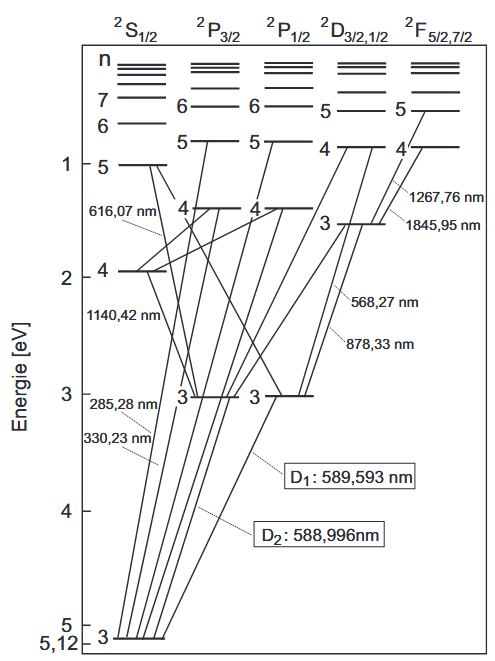
\includegraphics[width=8cm]{graphics/energieschemaNA.png}
    \caption{Energieschema und Photonübergänge im Natriumatom [Quelle: PAP2.1 Skript, S.124, 19.02.2024]}
    \label{fig:ergSchemaNA}
\end{figure}

\underline{Erwartete Linien für die 1. Nebenserie (md $\xrightarrow{}$ 3p)}

Zunächst wird angenommen, dass der Korrekturterm für die d-Energieniveaus gleich Null ist, wodurch sich die Wellenlängen ergeben als:

\begin{equation}
    \lambda_m = \frac{hc}{\frac{E_{\text{Ry}}}{m^2} - E_{\text{3p}}}
    \label{eq:1NS}
\end{equation}

Hierbei ist $h$ das Planck'sche Wirkungsquantum, $c$ die Lichtgeschwindigkeit, $E_{\text{Ry}} = -13,605$eV die Rydbergenergie, $m$ die Hauptquantenzahl des d-Niveaus und $E_{\text{3p}}$ die Energie des 3p Zustands.

\newpage

\underline{Erwartete Linien für die 2. Nebenserie (ms $\xrightarrow{}$ 3p)}

Mithilfe der bekannten D-Linie bei $\lambda = 589$nm mit dem Übergang 3p $\xrightarrow{}$ 3s lässt sich die Bindungsenergie des Grundzustands

\begin{equation}
    E_{\text{3s}} = E_{\text{3p}} - \frac{1}{\lambda} \ 1,2398 \cdot 10^3 \ \text{nm eV}
    \label{eq:ergGrundzustand}
\end{equation}

und daraus der Korrekturfaktor $\Delta_s$ bestimmen:

\begin{equation}
    E_{\text{3s}} = \frac{E_{\text{Ry}}}{(3 - \Delta_s)^2}
    \label{eq:KorrDelta_s}
\end{equation}

Somit kann man die erwarteten Wellenlängen bestimmen:

\begin{equation}
    \lambda_m = \frac{hc}{\frac{E_{\text{Ry}}}{(m - \Delta_s)^2} - E_{\text{3p}}}
    \label{eq:2NS}
\end{equation}

\hfill \\
\underline{Erwartete Linien für die Hauptserie (mp $\xrightarrow{}$ 3s)}

Mithilfe der Energie von 3p bestimmt man den Korrekturfaktor $\Delta_p$

\begin{equation}
    E_{\text{3p}} = \frac{E_{\text{Ry}}}{(3 - \Delta_p)^2}
    \label{eq:KorrDelta_p}
\end{equation}

und somit erneut die Wellenlängen:

\begin{equation}
    \lambda_m = \frac{hc}{\frac{E_{\text{Ry}}}{(m - \Delta_p)^2} - E_{\text{3s}}}
    \label{eq:HS}
\end{equation}

\subsection{Versuchsaufbau}

Das Kernstück des Versuchs ist das Gitterspektrometer, welches über eine Linse verschiedene Lichtquellen aufnehmen kann. Angeschlossen an einen Computer stellt dieser mit dem zugehörigen Programm die beobachteten Spektren dar und zeichnet diese auf.

\begin{figure}[!h]
    \centering
    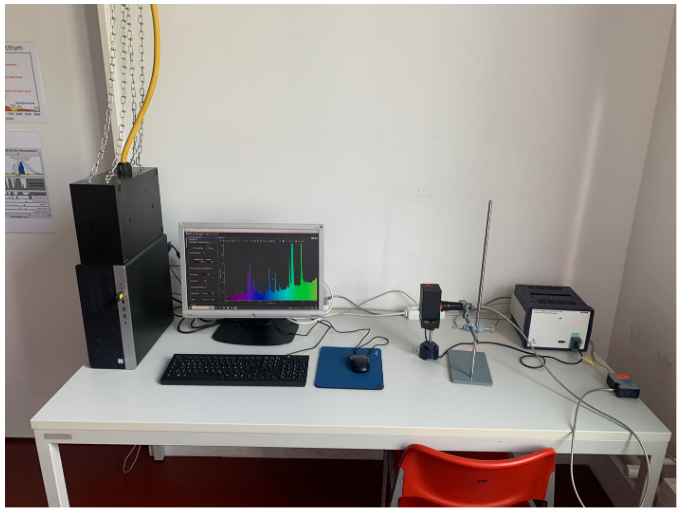
\includegraphics[width=8cm]{graphics/versuchsaufbau.png}
    \caption{Versuchsaufbau [Quelle: PAP2.1 Skript, S.124, 19.02.2024]}
    \label{fig:aufbau}
\end{figure}

%---------------VERSUCHSPROTOKOLL MIT MESSDATEN---------------
\newpage

\section{Versuchsprotokoll mit Messdaten}

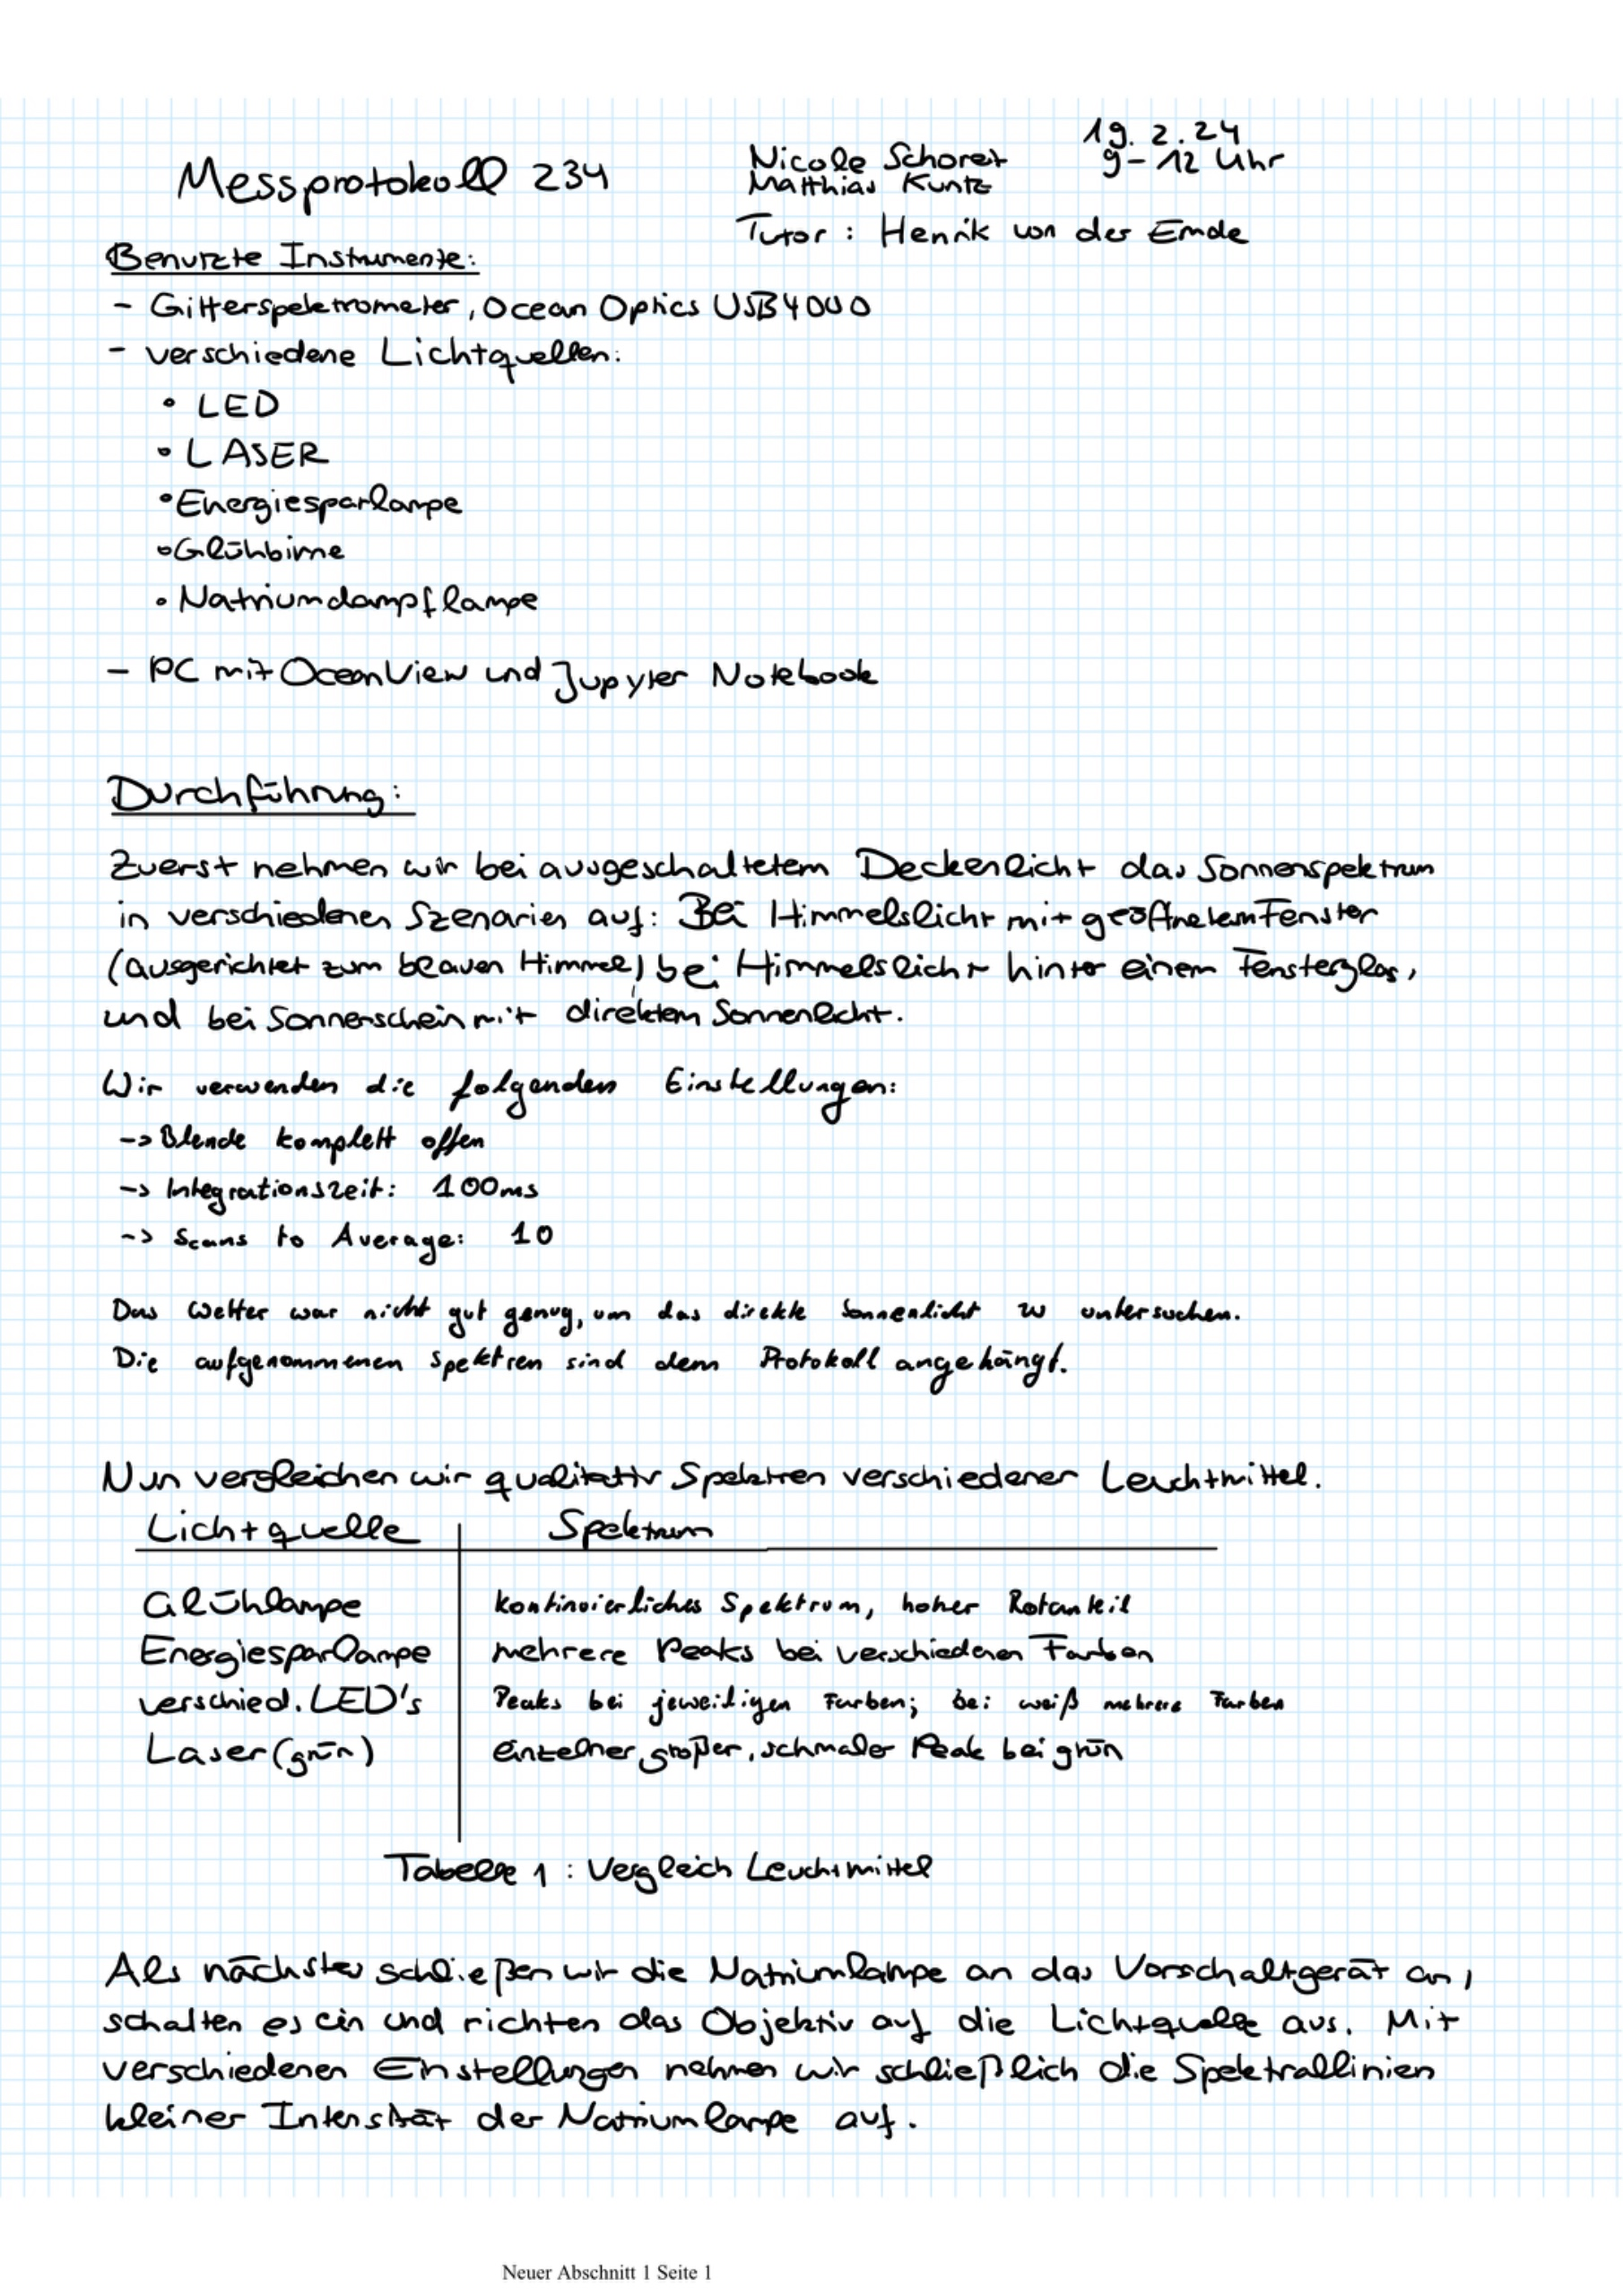
\includegraphics[width=\textwidth]{graphics/mess1.jpeg}
\newpage
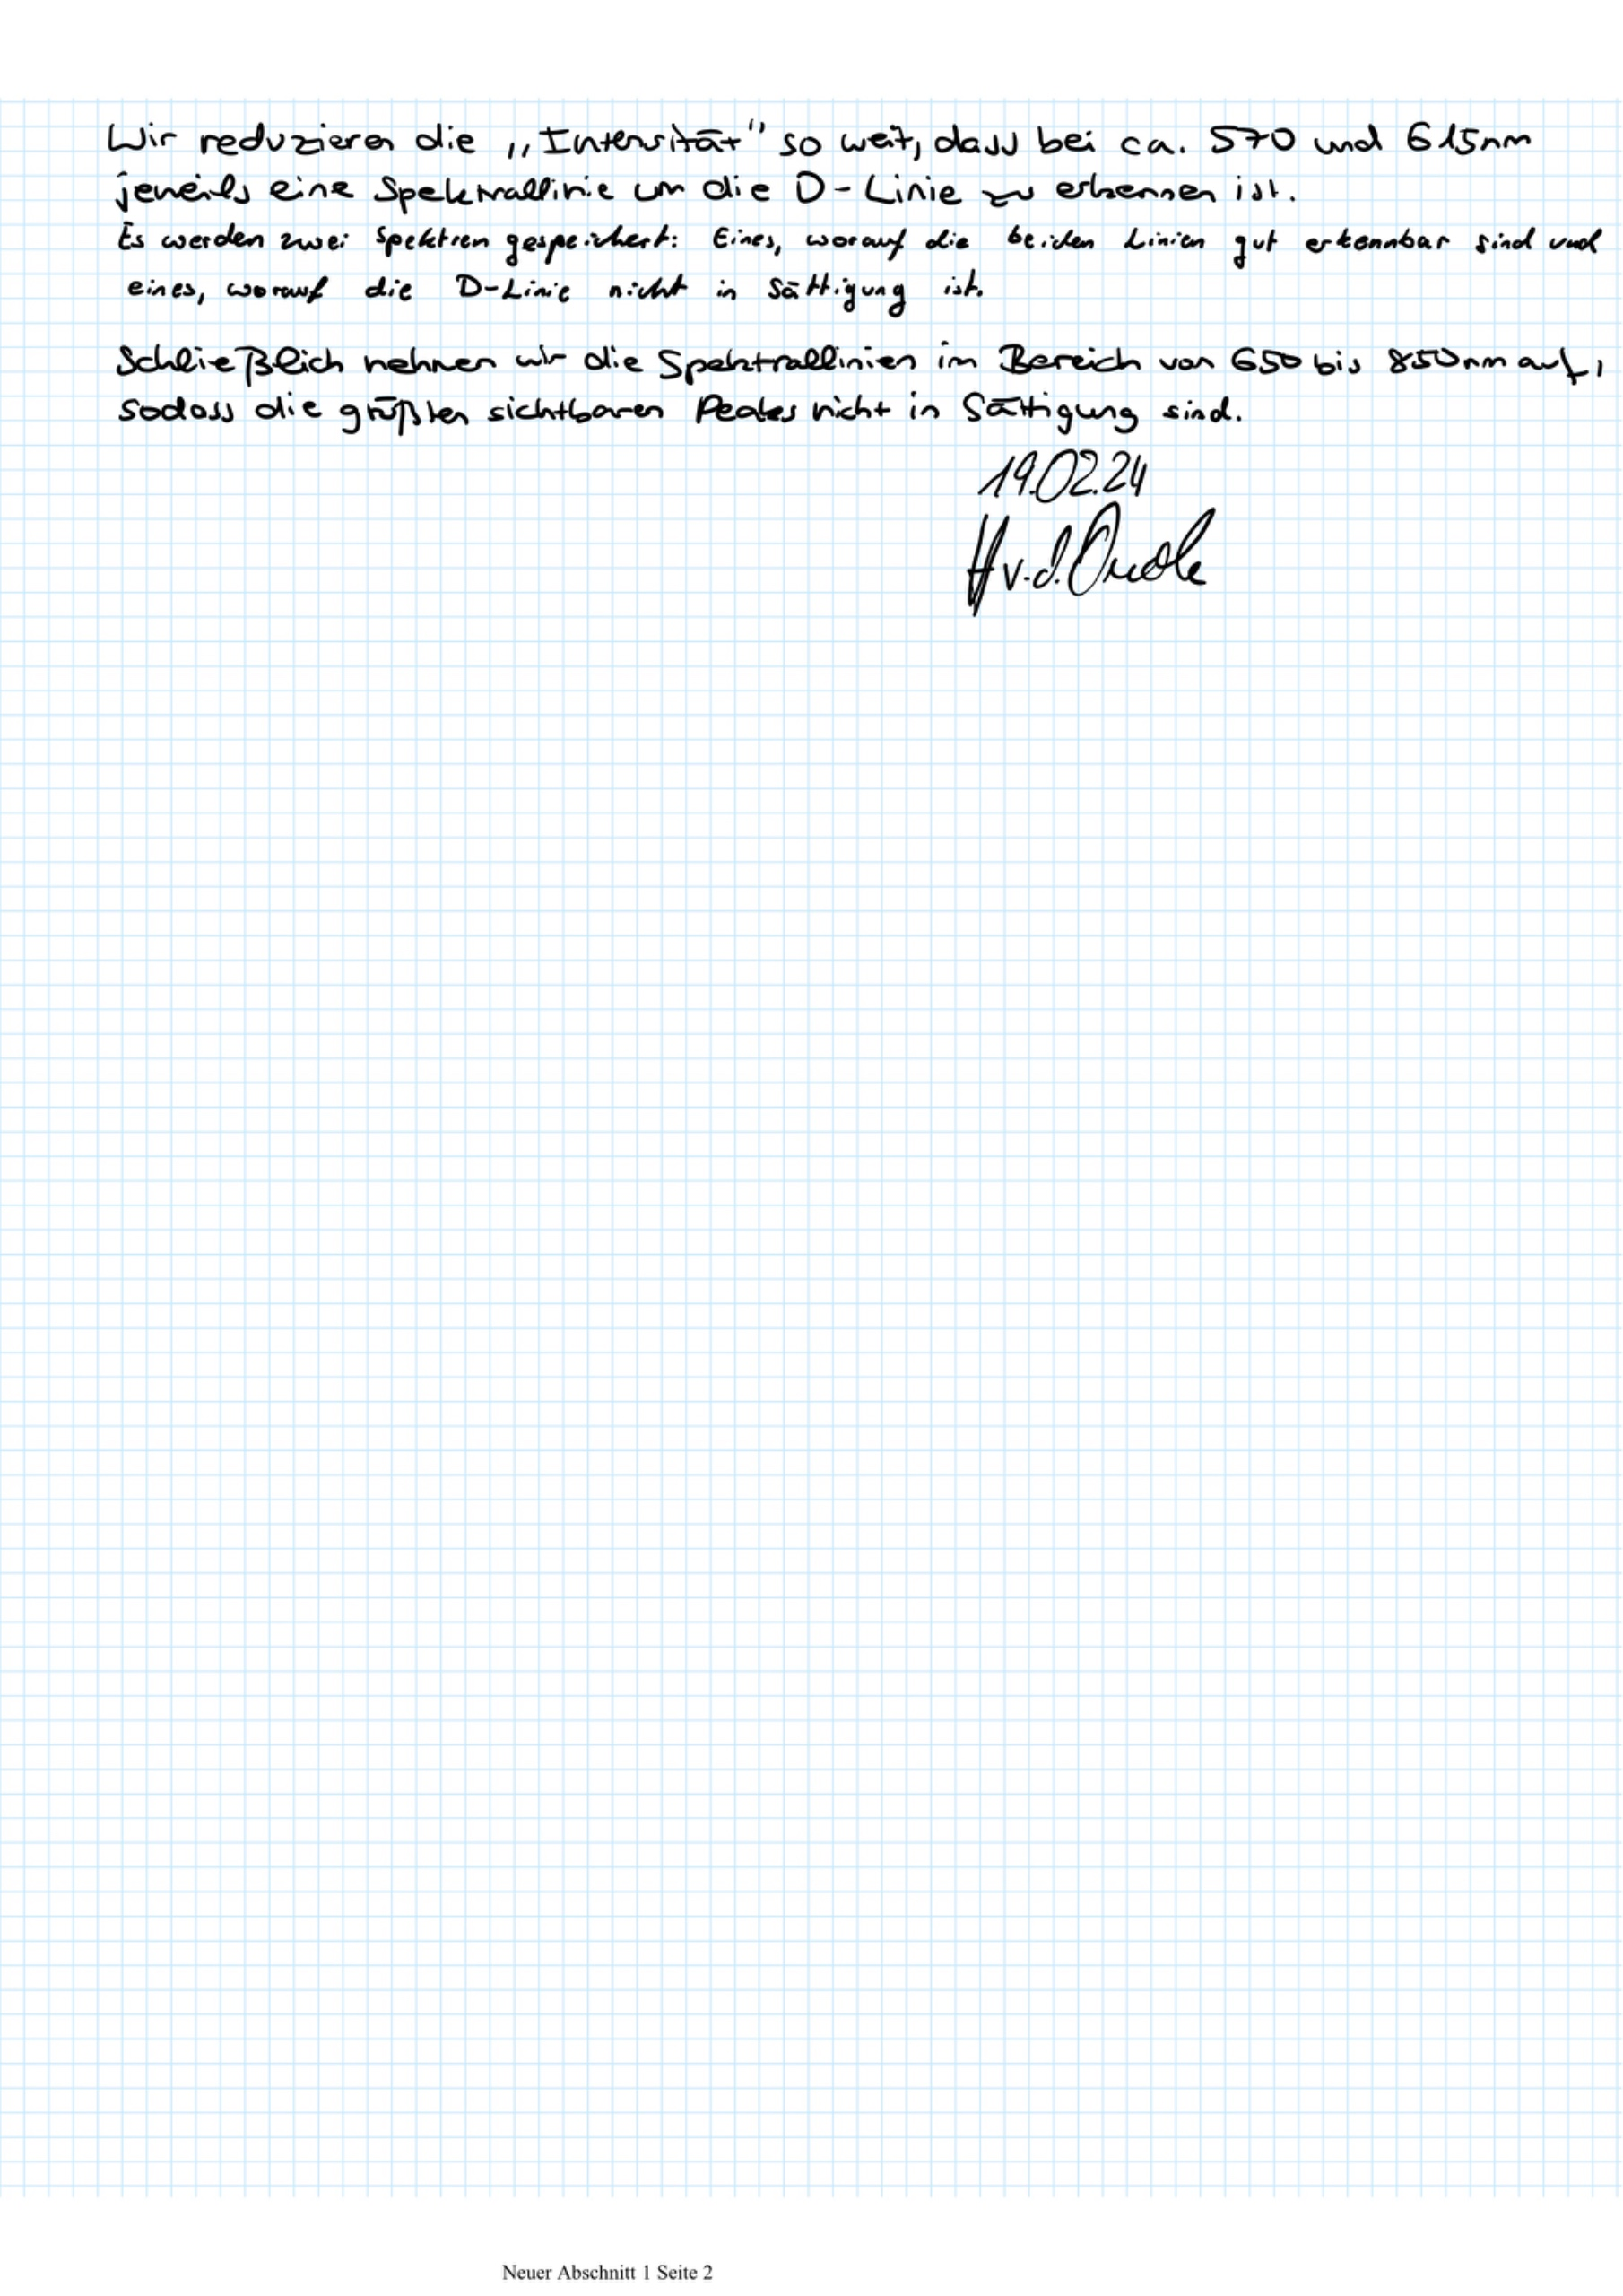
\includegraphics[width=\textwidth]{graphics/mess2.jpeg}
\newpage

\addtocounter{table}{1}

\phantom{.}

\begin{figure}[!h]
  \centering
  \subfloat[Himmel ohne Glas]{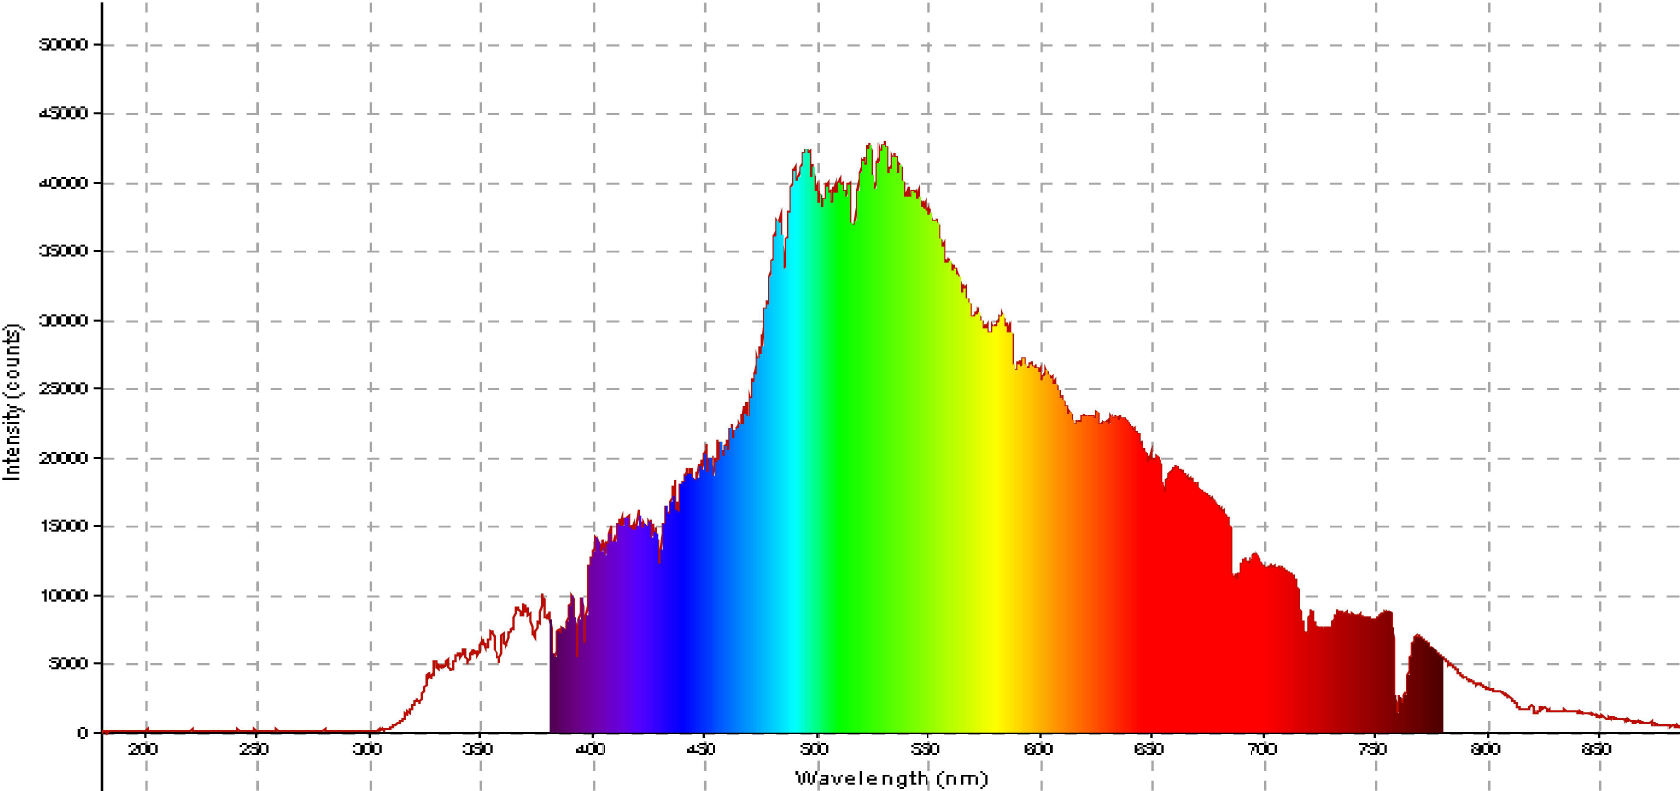
\includegraphics[width=0.48\textwidth]{graphics/HoF.png}\label{fig:OVHoF}}
  \hfill
  \subfloat[Himmel mit Glas]{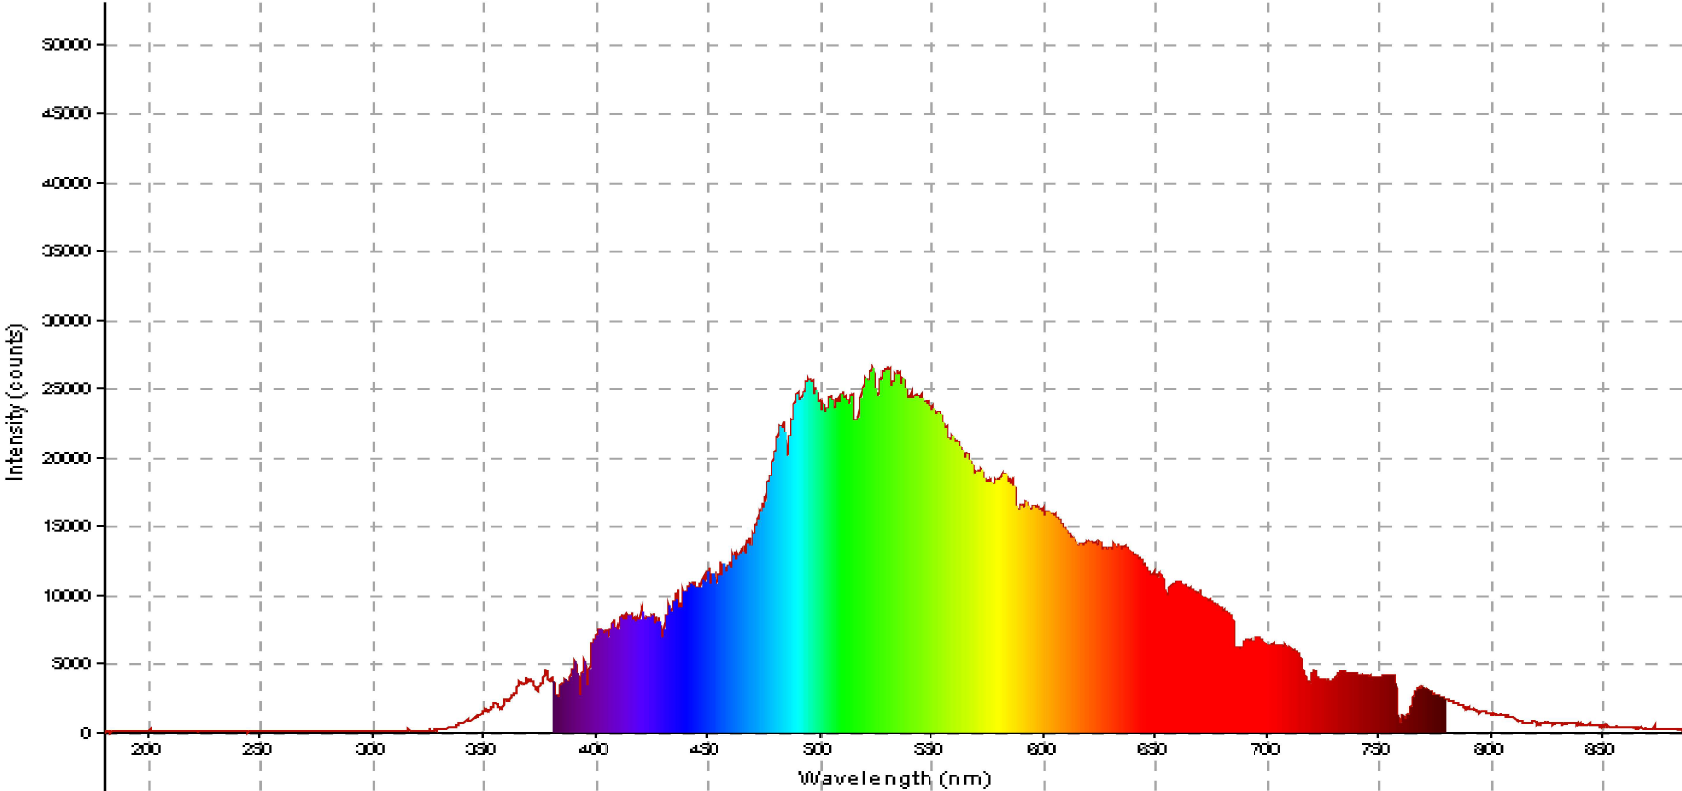
\includegraphics[width=0.48\textwidth]{graphics/HmF.png}\label{fig:OVHmF}}
  \caption{Gemessene Himmelspektren}
\end{figure}

\phantom{.}

\phantom{.}

\begin{figure}[!h]
  \centering
  \subfloat[Gelbe LED]{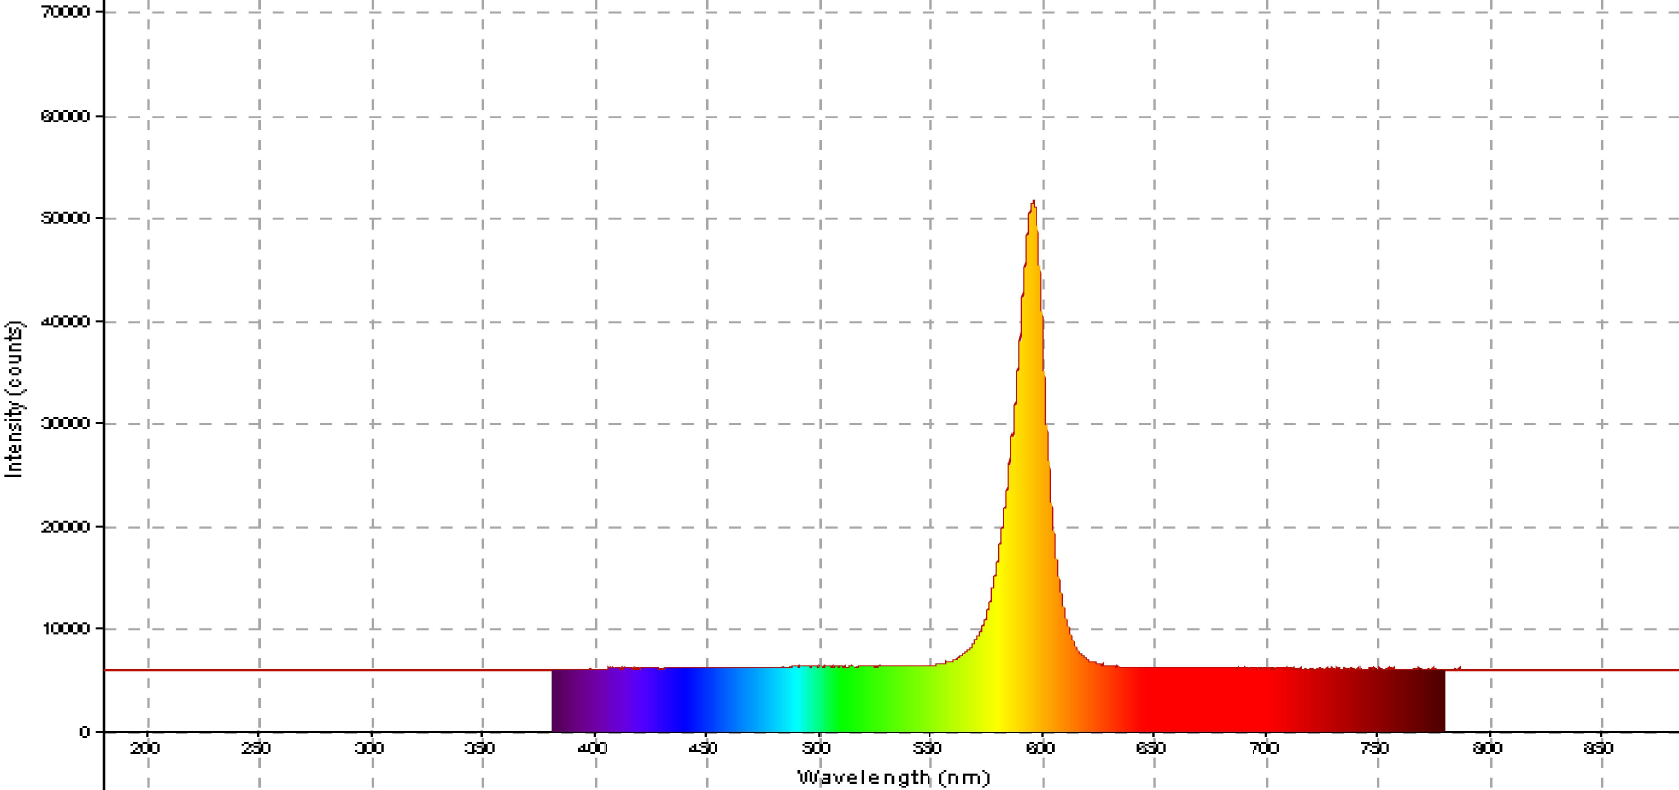
\includegraphics[width=0.48\textwidth]{graphics/vergleichspektren/gelbeLED.png}\label{fig:OVgelbeLED}}
  \hfill
  \subfloat[Rote LED]{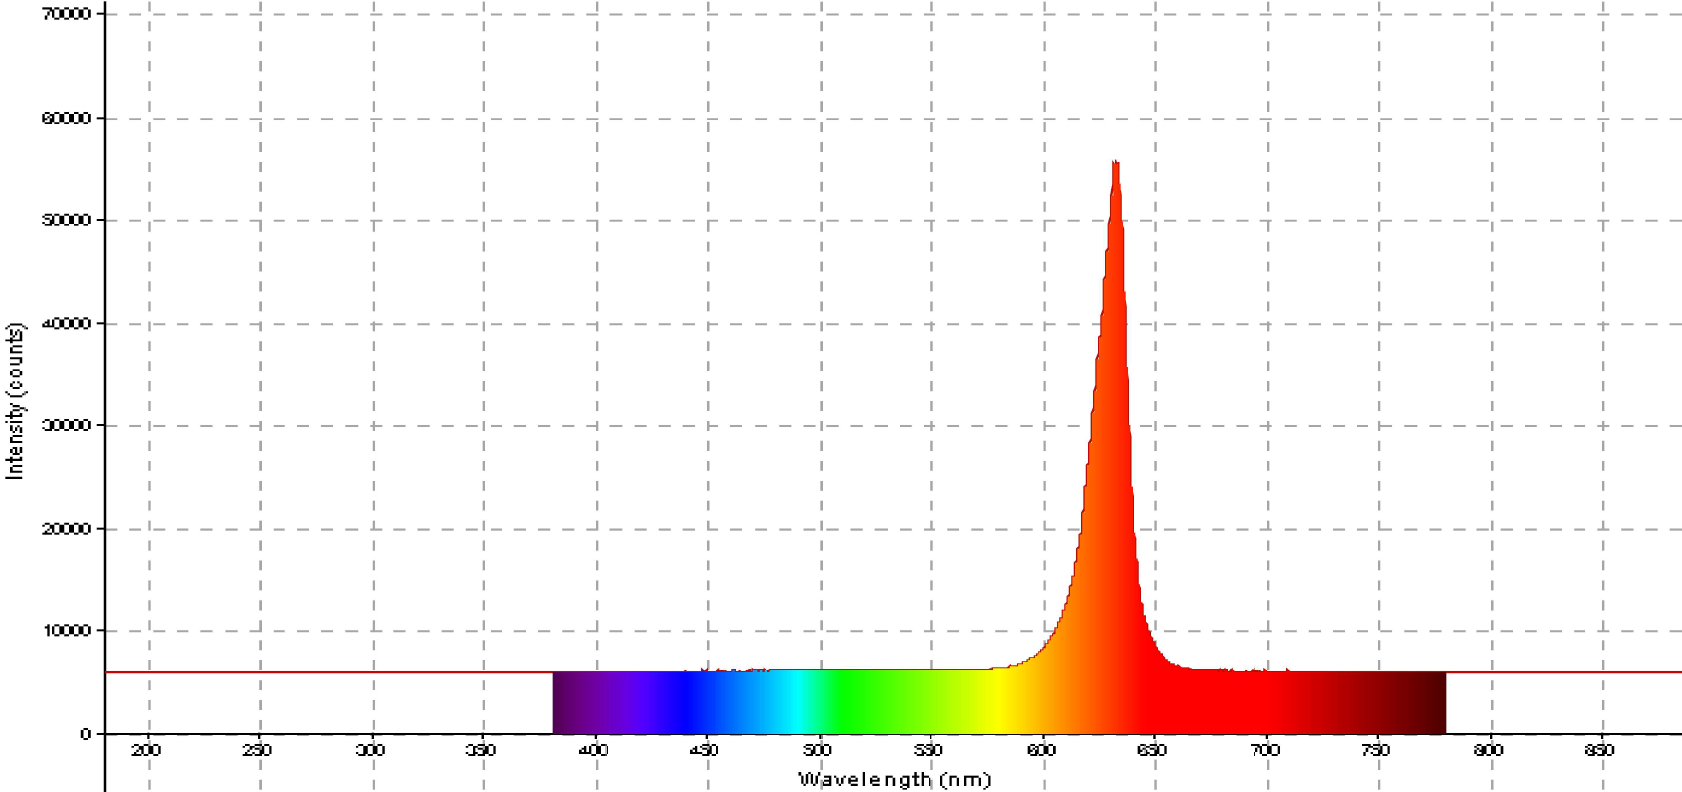
\includegraphics[width=0.48\textwidth]{graphics/vergleichspektren/roteLED.png}\label{fig:OVroteLED}}
  \hfill
  \subfloat[Weiße LED]{\includegraphics[width=0.48\textwidth]{graphics/vergleichspektren/weißeLED.png}\label{fig:OVweißeLED}}
  \hfill
  \subfloat[Grüner LASER]{\includegraphics[width=0.48\textwidth]{graphics/vergleichspektren/grünerLASER.png}\label{fig:OVgrünerLASER}}
  \hfill
  \subfloat[Glühlampe]{\includegraphics[width=0.48\textwidth]{graphics/vergleichspektren/glühlampe.png}\label{fig:OVglühlampe}}
  \hfill
  \subfloat[Energiesparlampe]{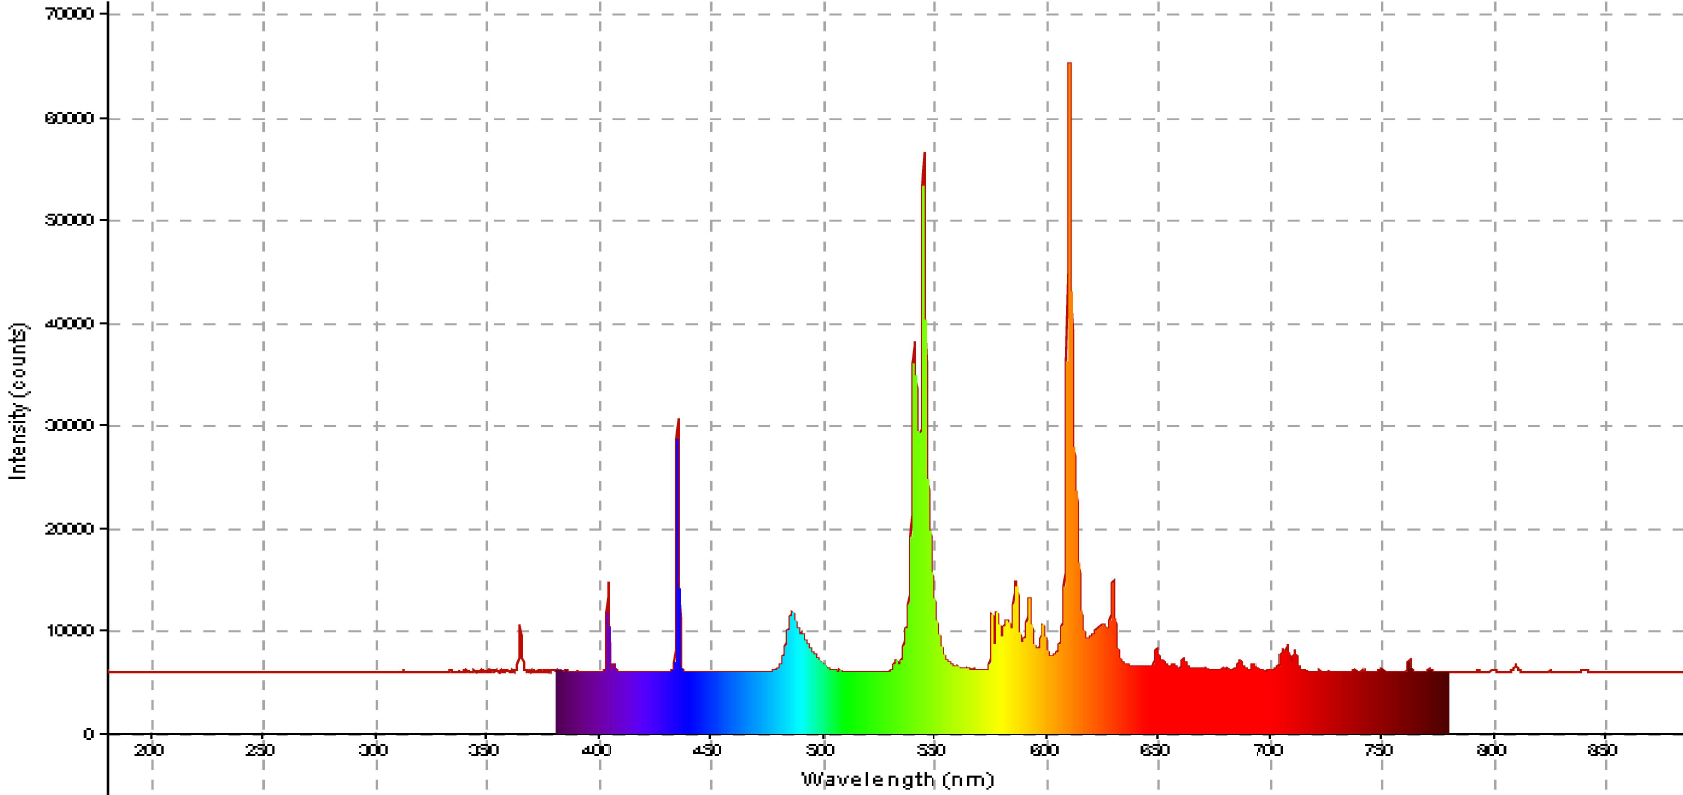
\includegraphics[width=0.48\textwidth]{graphics/vergleichspektren/energiesparlampe.png}\label{fig:OVenergiespar}}
  \caption{Gemessene Spektren verschiedener Leuchtkörper}
\end{figure}

\newpage
%-------------------------AUSWERTUNG-------------------------
\section{Auswertung}

In dieser Evaluation werden alle Fehler, sofern keine spezifische Angabe gemacht wird, mithilfe der Gauss'schen Fehlerfortpflanzung berechnet. Dies bedeutet, dass ein Wert $F$, der mit der Formel $f(a_1, ..., a_n)$ berechnet wird, den Fehler $\Delta F$ annimmt:

\begin{equation}
    \Delta F = \sqrt{\sum_n \left( \frac{\partial f}{\partial a_n} \cdot \Delta a_n \right)^2}.
\end{equation}

Des Weiteren erfolgen Signifikanztests von zwei Werten $a$ und $a'$ über die folgende Formel:

\begin{equation}
    \sigma = \frac{|a-a'|}{\sqrt{(\Delta a)^2 + (\Delta a')^2}}.
\end{equation}

Die Güte eines Fits wird mit der $\chi^2$-Summe bewertet:

\begin{equation}
    \chi^2 = \sum_i^N \left( \frac{\textit{Funktionswert}_i - \textit{Messwert}_i}{\textit{Fehler}_i} \right)^2
\end{equation}

Auch verwendet wird $\chi^2_{red} = \chi^2 / f$, wobei der Freiheitsgrad $f$ die Anzahl der Messwerte minus die Anzahl der Fitparameter ist. Der auf die Freiheitsgrade normierte Wert soll bei einem guten Fit ungefähr 1 sein.

\newpage

\subsection{Auswertung des Himmelhintergrunds mit und ohne Glas}

Wir beginnen, indem wir die Messungen vom Himmelslicht mit und ohne Fenster, Abbildung \ref{fig:OVHoF} \& \ref{fig:OVHmF}, in ein gemeinsames Diagramm plotten, zu sehen in Abbildung \ref{fig:HimmelVgl}. Es fällt auf, dass das Himmelslicht mit Fenster wie erwartet die gleiche Form hat wie das des direkten Himmels ohne Fenster, dafür aber eine schwächere Intensität aufweist.

Um einen quantitativen Vergleich der beiden Spektren zu vollziehen, berechnen wir mit Gleichung \ref{eq:absorp} den Absorptionskoeffizienten vom Glas und plotten die Ergebnisse für jede Wellenlänge in Abbildung \ref{fig:AbsGlas}. Es fällt auf, dass Glas in niedrigen Wellenlängen, ergo im UV-Bereich, fast alle Strahlung absorbiert, im Bereich des sichtbaren Lichts von etwa 400-650nm am durchlässigsten ist und zuletzt langsam mit größer werdenden Wellenlängen im Infrarotbereich wieder absorbierender wird. 

\phantom{.}

\begin{figure}[!p]
    \centering
    \resizebox{0.9\textwidth}{!}{
    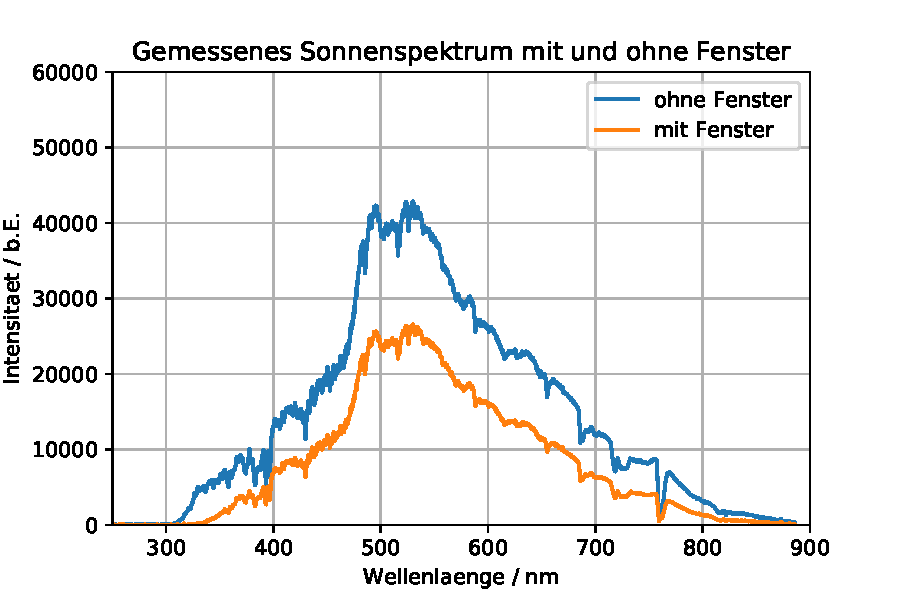
\includegraphics{graphics/outputs/Himmel_m_o_G.pdf}}
    \caption{Gemessenes Spektrum des Himmels}
    \label{fig:HimmelVgl}
\end{figure}

\phantom{.}

\begin{figure}[!p]
    \centering
    \resizebox{0.9\textwidth}{!}{
    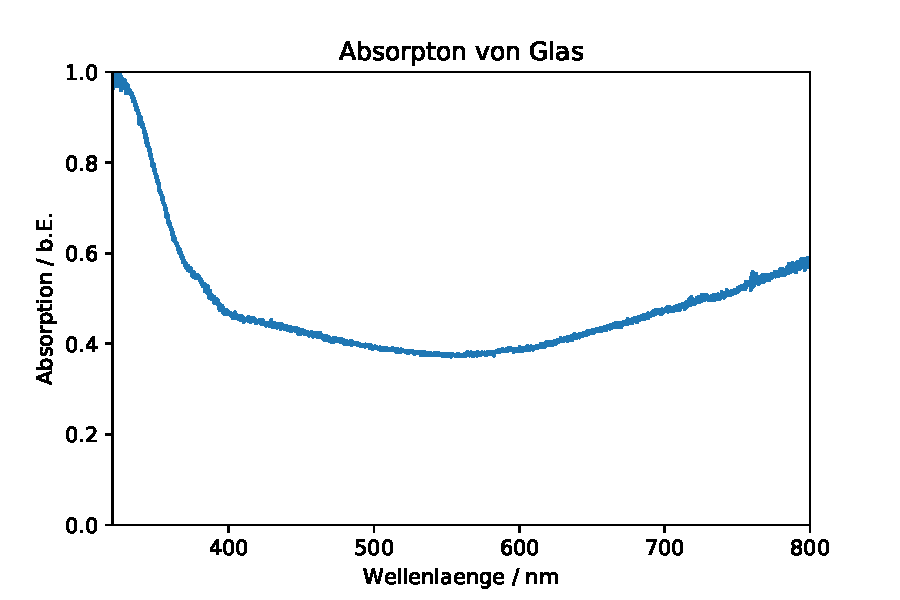
\includegraphics{graphics/outputs/Absorption_Glas.pdf}}
    \caption{Absorption von Glas}
    \label{fig:AbsGlas}
\end{figure}

\phantom{.}

\clearpage
\newpage
\subsection{Bestimmung der Fraunhoferlinien}

Aus dem gemessenen Spektrum des Himmels ohne Fenster sollen nun die Fraunhoferlinien bestimmt werden. Dazu lesen wir den Plot des Spektrums aus und messen die in der ersten Spalte von Tabelle \ref{tab:Fraunh} aufgelisteten Linien. Weitere sichtbare Linien im Spektrum sind das Resultat von Streustrahlung und somit nicht relevant.

Die notierten Linien werden mit den in Abbildung \ref{fig:fraunh_balmer} gegebenen Literaturwerten über einen Signifikanztest verglichen und das Resultat ebenso in der Tabelle verzeichnet.

\phantom{.}

\begin{table}[!h]
    \resizebox{\textwidth}{!}{
    \begin{tabular}{cccc}
    \hline
    \textbf{Gemessene Linie [nm]} & \textbf{Zuordnung} & \textbf{Literaturwert [nm]} & \textbf{Signifikanztest} \\ \hline
           $759,3 \pm 0,5$   &     A      &     759,4      &      0,2     \\
           $686,0 \pm 0,5$   &     B      &     686,7      &      1,4     \\
           $655,1 \pm 0,5$   &     C (H$_{\alpha}$)      &     656,3      &   2,4        \\
           $588,2 \pm 0,5$   &     D$_3$      &     587,6      &      1,2     \\
           $525,8 \pm 1,0$   &     E      &     527,0      &      1,2     \\
           $515,9 \pm 1,0$   &     b$_1$      &      518,4     &     2,5      \\
           $485,2 \pm 0,5$   &     F (H$_{\beta}$)      &      486,1     &   1,8        \\
           $433,4 \pm 0,5$   &     (H$_{\gamma}$)      &     434,0      &    1,2       \\
           $429,8 \pm 0,5$   &     G      &     430,8      &     2,0      \\
           $409,7 \pm 0,5$   &     (H$_{\sigma}$)      &     410,1      &    0,8       \\
           $396,5 \pm 0,5$   &     H      &     396,8      &      0,6     \\
           $393,0 \pm 0,5$   &     K      &     393,4      &      0,8     \\ \hline
    \end{tabular}}
    \caption{Gemessene Fraunhoferlinien und Zuordnung}
    \label{tab:Fraunh}
\end{table}

\phantom{.}

Alle gemessenen Wellenlängen liegen innerhalb der $3\sigma$-Umgebung und sind somit nicht signifikant. Nur die drei Werte der C, b$_1$ und G Linien weisen mit Sigmas von 2.4, 2.5 und 2.0 leicht erhöhte Abweichungen auf.

Zuletzt werden die vermessenen Linien noch in einem Diagramm mit dem Himmelspektrum eingetragen. Besonders hervorgehoben sind hier zum einen die Linien der Balmer-Serie des Wasserstoffs in lila und die Gelbe Helium D-Linie. Das Diagramm ist in Abbildung \ref{fig:HimmelMitLinien} zu sehen.

\begin{figure}[!h]
    \centering
    \resizebox{0.9\textwidth}{!}{
    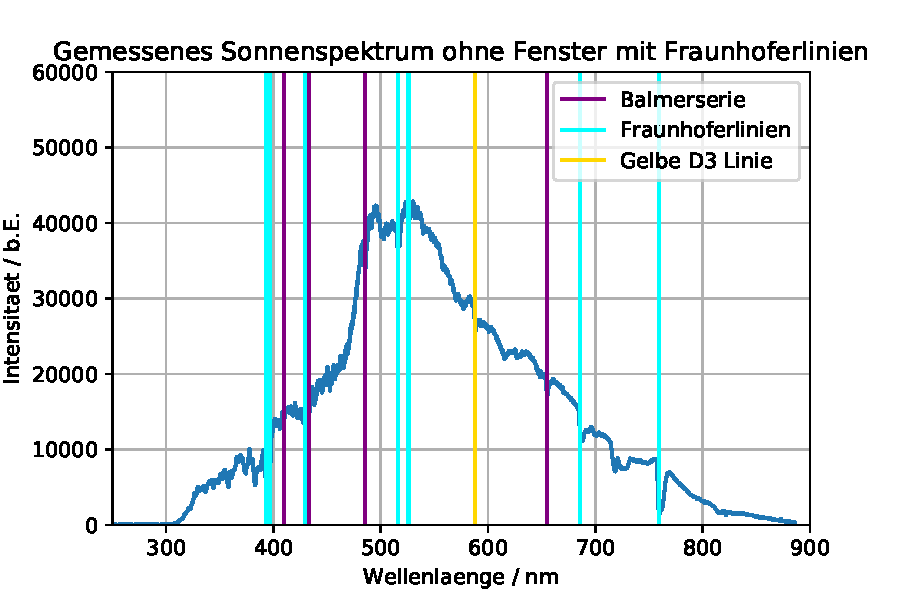
\includegraphics{graphics/outputs/Fraunhoferlinien.pdf}}
    \caption{Fraunhoferlinien im Himmelsspektrum}
    \label{fig:HimmelMitLinien}
\end{figure}
\clearpage

\newpage

\subsection{Vergleich verschiedener Lichtquellen}

Für einen Qualitativen Vergleich der Spektren der verschiedenen Leuchtkörper aus den Abbildungen \ref{fig:OVgelbeLED} bis \ref{fig:OVenergiespar} werden alle Spektren in ein gemeinsames Diagramm, Abbildung \ref{fig:VglLeuchtkörper}, gesetzt. Hier sind klar die starken Peaks der farbigen LEDs sowie des grünen Lasers zu erkennen. Auch die Energiesparlampe weist mehrere starke Peaks auf. Die weiße LED hingegen hat ein eher kontinuierlicheres Spektrum und die Glühlampe hat eine viel geringere Intensität als alle anderen mit einem sehr hohen Infrarotanteil. 

Die Lichtquellen, deren Spektren einen größeren Rotanteil haben, wie beispielsweise die Glühlampe sowie die rote und gelbe LED, senden Warmlicht aus. Die mit einem größeren Blauanteil, wie die Weiße LED mit dem großen Peak bei etwa 450nm, senden hingegen Kaltlicht aus. 

\phantom{.}

\begin{figure}[!h]
    \centering
    \resizebox{0.9\textwidth}{!}{
    \includegraphics{graphics/outputs/Leuchtkörper-2.pdf}}
    \caption{Vergleich der sechs Leuchtkörper}
    \label{fig:VglLeuchtkörper}
\end{figure}


\newpage

\subsection{Analyse des Natriumspektrums}

\underline{Zuordnung der Linien zu den Serien}

Wir beginnen, indem wir die aufgenommenen Spektren, dargestellt in Abbildung \ref{fig:alleNatriumspektren}, auszuwerten, indem wir die Wellenlängen der klar sichtbaren Peaks vermessen und den Fehler anhand der Halbwertsbreite der Peaks abschätzen.

Anschließend berechnen wir wie in Kapitel \ref{DasNatriumspektrum} erläutert die erwarteten Wellenlängen der 1. Nebenserie für $m = 0$ bis $m = 12$, der 2. Nebenserie für $m = 4$ bis $m = 9$ und der Hauptserie für $m = 4$ und $m = 5$ sowie deren Fehler über die Fehlerfortpflanzung: 

\begin{equation}
    \text{d} \lambda_{NS1} = \left| \frac{hc}{(E_{Ry}/m^2 - E_{3p})^2} \text{d}E_{3p} \right|  
\end{equation}

\begin{equation}
    \begin{split}
        \text{d} \lambda_{NS2} &= \Biggl[ \Biggl(\frac{2 hc E_{Ry} (m-\Delta_s)}{(E_{Ry} - E_{3p} (m-\Delta_s)^2)^2} \text{d}\Delta_s \Biggr)^2 \\
        &+ \Biggl( \frac{hc}{(E_{Ry}/(m - \Delta_s)^2 - E_{3p})^2} \text{d}E_{3p} \Biggr)^2 \Biggr]^{1/2}
    \end{split}
\end{equation}

\begin{equation}
    \begin{split}
        \text{d} \lambda_{HS} &= \Biggl[ \Biggl(\frac{2 hc E_{Ry} (m-\Delta_p)}{(E_{Ry} - E_{3s} (m-\Delta_p)^2)^2} \text{d}\Delta_p \Biggr)^2 \\
        &+ \Biggl( \frac{hc}{(E_{Ry}/(m - \Delta_p)^2 - E_{3s})^2} \text{d}E_{3s} \Biggr)^2 \Biggr]^{1/2}
    \end{split}
\end{equation}

Dazu berechnen wir zunächst mit Gleichung \ref{eq:1NS} die Energie des 3p Zustands $E_{3p}$, indem wir der gemessenen Linie im Bereich von 819nm die Quantenzahl $m = 3$ zuordnen. Wir erhalten:

\begin{equation}
    E_{3p} = (-3,027 \pm 0,004) \text{eV}
\end{equation}

Damit können wir bereits alle erwarteten Linien der 1. Nebenserie berechnen. Die Ergebnisse sowie die zugeordneten Linien sind mitsamt Signifikanztest in Tabelle \ref{tab:1NS} dargestellt. Bei den freien Felder in der Tabelle konnte dem erwarteten Wert keine gemessene Linie eindeutig genug zugeordnet werden.

\phantom{.}

\begin{table}[!h]
    \centering
    \resizebox{\textwidth}{!}{
    \begin{tabular}{cccc}
        \hline
        \textbf{QZ} & \textbf{erwartete Linie} [nm] & \textbf{zugeordnete Linie} [nm] & \textbf{Signifikanztest} \\ \hline
          3 & 817,9 $\pm$ 2,2 & 817,9 $\pm$ 2,2 & 0 (Referenz) \\
          4 & 569,5 $\pm$ 1,1 & 567 $\pm$ 3 & 0,8 \\
          5 & 499,3 $\pm$ 0,8 & 496,9 $\pm$ 1,7 & 1,2 \\
          6 & 467,9 $\pm$ 0,7 & 465,8 $\pm$ 1,0 & 1,7 \\
          7 & 450,9 $\pm$ 0,7 & 449 $\pm$ 3 & 0,6 \\
          8 & 440,4 $\pm$ 0,6 & - & - \\
          9 & 433,6 $\pm$ 0,6 & 432,8 $\pm$ 1,0 & 0,7 \\
         10 & 428,8 $\pm$ 0,6 & 429,3 $\pm$ 0,5 & 0,7 \\
         11 & 425,3 $\pm$ 0,6 & 426,2 $\pm$ 1,2 & 0,7 \\
         12 & 422,7 $\pm$ 0,6 & - & - \\ \hline
    \end{tabular}}
    \caption{Zugeornete Linien der 1. Nebenserie}
    \label{tab:1NS}
\end{table}

\phantom{.}

Für die erwarteten Linien der 2. Nebenserie bestimmen wir via Gleichung \ref{eq:ergGrundzustand} die Energie des Grundzustands

\begin{equation}
    E_{3s} = (-5,132 \pm 0,004) \text{eV}
\end{equation}

sowie mit Gleichung \ref{eq:KorrDelta_s} den Korrekturfaktor

\begin{equation}
    \Delta_s = 1,3719 \pm 0,0006
\end{equation}

und schlussendlich damit die erwarteten Wellenlängen mit Gleichung \ref{eq:2NS}. Die Ergebnisse sind in Tabelle \ref{tab:2NS} erneut mit den zugeordneten Wellenlängen sowie dem Signifikanztest.

\phantom{.}

\begin{table}[!h]
    \centering
    \resizebox{\textwidth}{!}{
    \begin{tabular}{cccc}
        \hline
        \textbf{QZ} & \textbf{erwartete Linie} [nm] & \textbf{zugeordnete Linie} [nm] & \textbf{Signifikanztest} \\ \hline
         4 & 1172 $\pm$ 5 & - & - \\
         5 &  621,8 $\pm$  1,3 & 614,5 $\pm$ 1,3 & 4 \\
         6 &  518,2 $\pm$  0,9 & 517,3 $\pm$ 1,0 & 0,7 \\
         7 &  477,2 $\pm$  0,8 & 474,2 $\pm$ 0,7 & 2,9 \\
         8 &  456,2 $\pm$  0,7 & 454,4 $\pm$ 0,7 & 1,8 \\ \hline
    \end{tabular}}
    \caption{Zugeornete Linien der 2. Nebenserie}
    \label{tab:2NS}
\end{table}

\phantom{.}
\newpage

Zu guter Letzt wird für die Berechnung der Hauptserie der Korrekturfaktor

\begin{equation}
    \Delta_p = 0,8801 \pm 0,0014
\end{equation}

mittels Gleichung \ref{eq:KorrDelta_p} bestimmt, woraufhin durch Gleichung \ref{eq:HS} die zwei erwarteten Linien bestimmt werden können. Die Ergebnisse mit Zuordnung finden sich in Tabelle \ref{tab:HS}.

\phantom{.}

\begin{table}[!h]
    \centering
    \resizebox{\textwidth}{!}{
    \begin{tabular}{cccc}
        \hline
        \textbf{QZ} & \textbf{erwartete Linie} [nm] & \textbf{zugeordnete Linie} [nm] & \textbf{Signifikanztest} \\ \hline
         4 & 332,0 $\pm$ 0,4 & 329,8 $\pm$ 1,5 & 1,4 \\
         5 & 286,27 $\pm$  0,27 & 284,2 $\pm$ 0,6 & 3 \\ \hline
    \end{tabular}}
    \caption{Zugeornete Linien der Hauptserie}
    \label{tab:HS}
\end{table}

\phantom{.}

Es ist anzumerken, dass die meisten zugeordneten Wellenlängen aller drei Serien in einem insignifikanten Sigmabereich liegen. Die Linie bei höhrem Sigma der 2. Nebenserie bleibt als Messwert stehen, damit für den nächsten Schritt genug Werte für den Fit bleiben.

\begin{figure}[p]
  \centering
  \subfloat[Bereich 400-540nm]{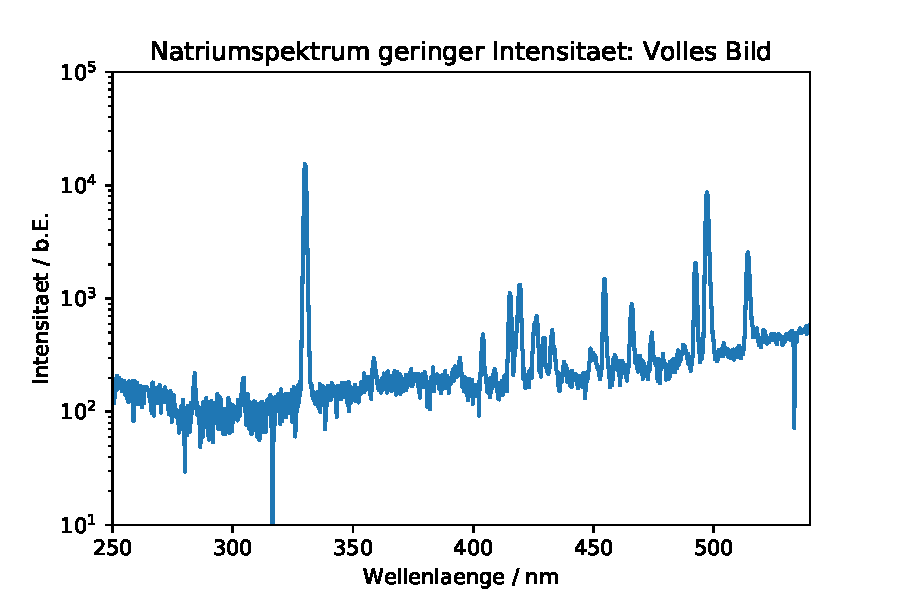
\includegraphics[width=0.48\textwidth]{graphics/outputs/NA_low_full.pdf}\label{fig:NA_low}}
  \hfill
  \subfloat[Bereich 650-800nm]{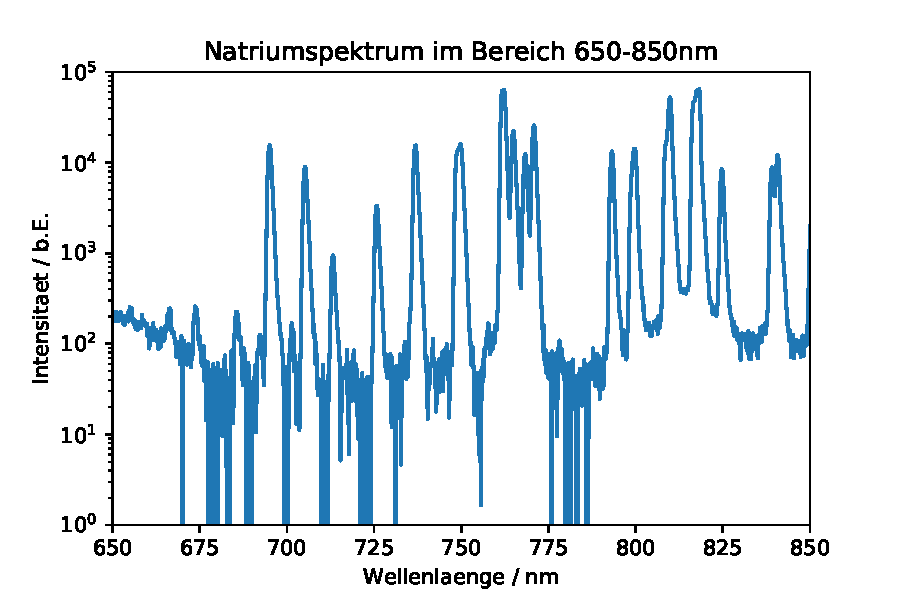
\includegraphics[width=0.48\textwidth]{graphics/outputs/NA_high.pdf}\label{fig:NA_high}}
  \hfill
  \subfloat[D-Linie - Volles Bild]{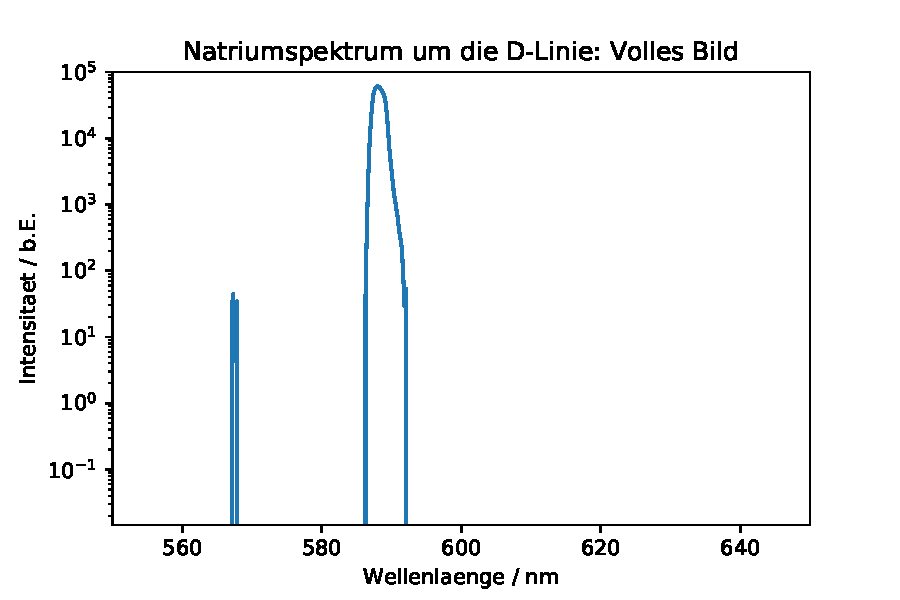
\includegraphics[width=0.48\textwidth]{graphics/outputs/NA_D_full.pdf}\label{fig:NA_D_full}}
  \hfill
  \subfloat[D-Linie - Zoom]{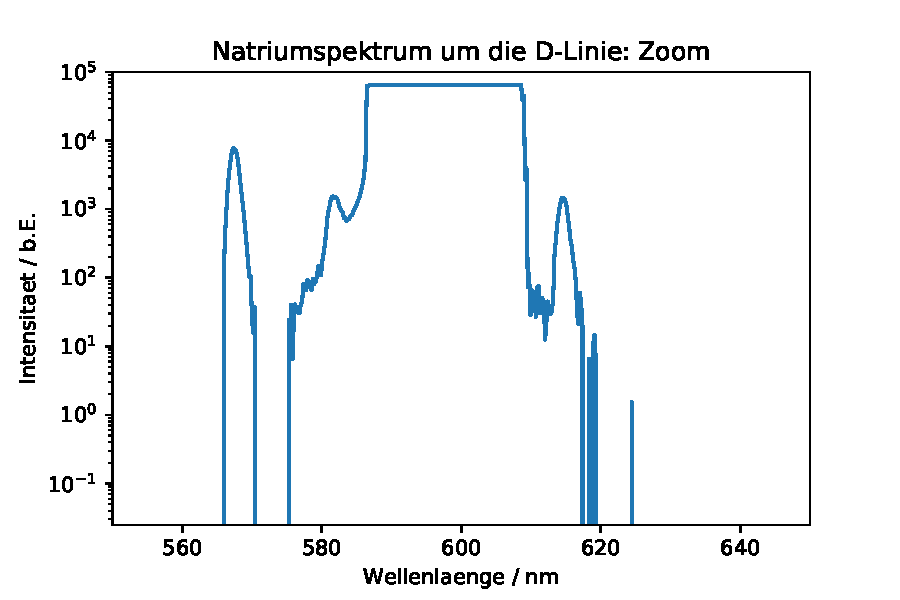
\includegraphics[width=0.48\textwidth]{graphics/outputs/NA_D_zoom.pdf}\label{fig:NA_D_zoom}}
  \hfill
  \caption{Gemessene Spektren der Natriumlampe}
  \label{fig:alleNatriumspektren}
\end{figure}

\clearpage
\newpage

\underline{Bestimmung der Serienergien und der l-abhängigen Korrekturfaktoren}

Wir wollen nun aus den zugeordneten Wellenlängen die Rydbergenergie $E_{Ry}$, die Energie des 3p Zustands $E_{3p}$, sowie die Korrekturterme $\Delta_d$ und $\Delta_s$ bestimmen. Dazu plotten wir die zugeordneten Wellenlängen der beiden Nebenserien in Abhängigkeit der zugehörigen Quantenzahl und fitten jeweils eine Funktion mit den zu bestimmenden Werten als Parameter an.

Wir beginnen mit der 1. Nebenserie und fitten die Funktion

\begin{equation}
    \lambda_m = \frac{hc}{\frac{E_{Ry}}{(m - \Delta_d)^2} - E_{3p}}
\end{equation}

wobei $hc$ weiterhin Planck'sches Wirkungsquantum sowie die Lichtgeschwindigkeit sind. Der Plot mit Fit ist in Abbildung \ref{fig:1NS} zu sehen. 



Die Güte des Fits sowie die Fitwahrscheinlichkeit betragen:

\begin{equation}
    \begin{split}
        \chi^2_1 &= 1,60 \\
        \chi^2_{red,1} &= 0,32 \\
        \text{Wsk.}_1 &= 90,0 \%
    \end{split}
\end{equation}

Die vom Fit berechneten Werte werden in Tabelle \ref{tab:Fit1} mit den Literaturwerten beziehungsweise den zuvor berechneten Werten verglichen.

\phantom{.}

\begin{table}[!h]
    \centering
    \begin{tabular}{c|ccc}
        \hline
        \textbf{} & \textbf{Fit-Wert} & \textbf{Vergleichswert} & \textbf{Signifikanztest} \\ \hline
        $\mathbf{E_{Ry}}$ [eV] &     $-12,17 \pm 0,28$      &     $ -13,605 $      &     5,1      \\
        $\mathbf{E_{3p}}$ [eV] &     $-3,015 \pm 0,003$      &      $ -3,027 \pm 0,004 $     &    2,4       \\
        $\mathbf{\Delta_d}$ &      $0,15 \pm 0,03$     &     $ 0 $      &      4,9     \\ \hline
    \end{tabular}
    \caption{Fit-Werte der 1. Nebenserie}
    \label{tab:Fit1}
\end{table}

\phantom{.}

Hier ist auffällig, dass $\chi^2_{red,1}$ auffällig vom erwünschten Wert 1 abweicht. Außerdem weisen die Fit-Werte praktisch alle signifikante Abweichungen vom Vergleichswert auf. Nur der Wert für $E_{3p}$ liegt innerhalb der $3\sigma$-Umgebung, ist aber auch erhöht.
\newpage

Für die 2. Nebenserie fitten wir die Funktion

\begin{equation}
    \lambda_m = \frac{hc}{\frac{E_{Ry}}{(m - \Delta_s)^2} - E_{3p}},
\end{equation}

was in Abbildung \ref{fig:2NS} dargestellt ist.

Hier betragen die Güte des Fits sowie die Fitwahrscheinlichkeit:

\begin{equation}
    \begin{split}
        \chi^2_2 &= 4,46 \\
        \chi^2_{red,2} &= 4,46 \\
        \text{Wsk.}_2 &= 3,0 \%
    \end{split}
\end{equation}

Auch hier Vergleichen wir die Fit-Werte mit den zuvor gegebenen, zu sehen in Tabelle \ref{tab:Fit2}.

\phantom{.}

\begin{table}[!h]
    \centering
    \begin{tabular}{c|ccc}
        \hline
        \textbf{} & \textbf{Fit-Wert} & \textbf{Vergleichswert} & \textbf{Signifikanztest} \\ \hline
        $\mathbf{E_{Ry}}$ [eV] &     $-15 \pm 3$      &     $ -13,605 $      &     0,6      \\
        $\mathbf{E_{3p}}$ [eV] &     $-3,07 \pm 0,05$      &      $ -3,027 \pm 0,004 $     &    0,8       \\
        $\mathbf{\Delta_s}$ &      $1,1 \pm 0,4$     &     $ 1,3719 \pm 0,0006 $      &      0,7     \\ \hline
    \end{tabular}
    \caption{Fit-Werte der 2. Nebenserie}
    \label{tab:Fit2}
\end{table}

\phantom{.}

Zwar liegen alle Fit-Werte innerhalb insignifikanter Abweichungen, jedoch ist dies vor allem beim Wert für $E_{Ry}$ hauptsächlich dem großen Fehler des Fit-Werts geschuldet. Zudem ist $\chi^2_{red,2}$ deutlich vom gewünschten Wert entfernt.

Allgemein lässt sich also schlussfolgern, dass ein grundlegender systematischer Fehler bei unseren aufgezeichneten Daten vorliegen muss.

\newpage

\begin{figure}[!p]
    \centering
    \resizebox{0.9\textwidth}{!}{
    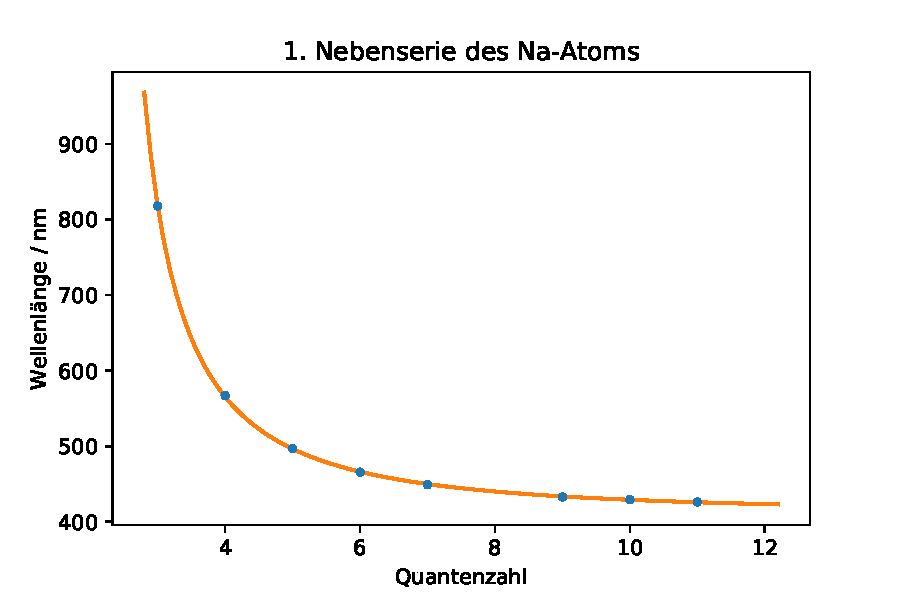
\includegraphics{graphics/outputs/NS1_fit.pdf}}
    \caption{1. Nebenserie des Natriumatoms}
    \label{fig:1NS}
\end{figure}

\begin{figure}[!p]
    \centering
    \resizebox{0.9\textwidth}{!}{
    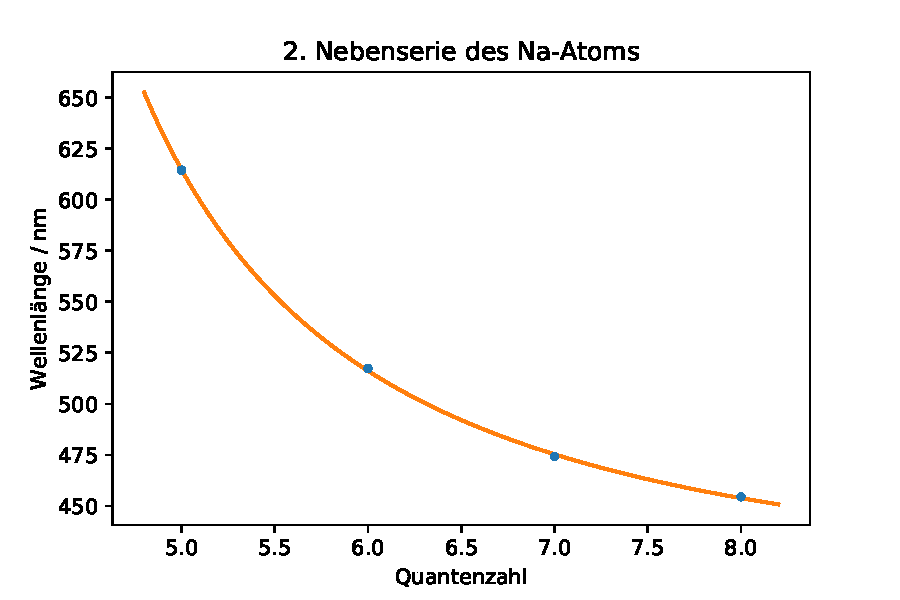
\includegraphics{graphics/outputs/NS2_fit.pdf}}
    \caption{2. Nebenserie des Na-Atoms}
    \label{fig:2NS}
\end{figure}

\clearpage
\newpage
%---------------PRÄSENTATION DER ENDERGEBNISSE---------------
\section{Zusammenfassung der Endergebnisse}

In diesem Versuch haben wir Spektren von verschiedenen Quellen aufgenommen und ausgwertet.

Angefangen beim Himmelsspektrum analysierten wir den Unterschied zwischen direkter Betrachtung und Beobachtung durch ein Fenster, indem wir die Absorbtion vom Glas bestimmten. Daraufhin entnahmen wir dem gemessen Spektrum ohne Fenster die Fraunhoferlinien, welche alle innerhalb insignifikanter Abweichungen von Literaturwerten lagen. 

Anschließend verglichen wir qualitativ die Spektren verschiedener Leuchtkörper wie Lampen, LEDs und einem Laser. Hier wurde der Unterschied zwischen kontinuierlichen und diskreten Spektren sichtbar und die Quellen wurden in Warm- und Kaltlicht unterteilt.

Am ausfühlichsten fand die Auswertung des Spektrums einer Natriumlampe statt. Aus den verschiedenen aufgenommenen Bereichen wurden alle deutlich sichtbaren Peaks ausgelesen und den berechneten erwarteten Linien der Hauptserie sowie der 1. und 2. Nebenserie zugeordnet. Dazu wurde die Energie des Zustands 3p und des Grundzustands 3s, sowie die Korrekturfaktoren $\Delta_s$ und $\Delta_p$ berechnet:

\begin{equation}
    \begin{split}
        E_{3p} &= (-3,027 \pm 0,004) \text{eV} \\
        E_{3s} &= (-5,132 \pm 0,004) \text{eV} \\
        \Delta_s &= 1,3719 \pm 0,0006 \\
        \Delta_p &= 0,8801 \pm 0,0014
    \end{split}
\end{equation}

Hierbei lagen die meisten Wellenlängen, die eindeutig zugeordnet werden konnten, innerhalb der $3\sigma$-Umgebung. Leider konnten bei der 1. sowie bei der 2. Nebenserie jeweils zwei Wellenlängen nicht eindeutig genug zugeordnet werden. 

Zuletzt wurden die zugeordneten Wellenlängen der beiden Nebenserien genutzt, um wiederum mithilfe eines Fits die Rydbergenergie und die Energie des 3p-Zustands, sowie die beiden Korrekturfaktoren $\Delta_d$ und $\Delta_s$ zu bestimmen. Die 1. Nebenserie ergab mit einer Güte von $\chi^2_{red,1} = 0,32$ die Werte:

\begin{equation}
    \begin{split}
        E_{Ry} &= (-12,17 \pm 0,28) \text{eV} \\
        E_{3p} &= (-3,015 \pm 0,003) \text{eV} \\
        \Delta_d &= 0,15 \pm 0,03
    \end{split}
\end{equation}

Hierbei weisen die Werte von $E_{Ry}$ und $\Delta_d$ signifikante Abweichungen von den Vergleichswerten auf.

Der Fit der 2. Nebenserie ergab mit einer Güte von $\chi^2_{red,2} = 4,46$ folgende Ergebnisse:

\begin{equation}
    \begin{split}
        E_{Ry} &= (-15 \pm 3) \text{eV} \\
        E_{3p} &= (-3,07 \pm 0,05) \text{eV} \\
        \Delta_s &= 1,1 \pm 0,4
    \end{split}
\end{equation}

Diese Werte liegen alle innerhalb der $1\sigma$-Umgebung der Referenzen.

\newpage
%---------------ZUSAMMENFASSUNG UND DISKUSSION---------------
\section{Diskussion}

Die Ergebnisse der Auswertung des Himmelslichts sowie die Analyse der Verschiedenen Lichtquellen erfüllten die vorherigen Erwartungen. Der Vergleich der direkten Messung mit der durchs Fenster entsprach der Theorie, die bestimmte Absorption des Glases ergibt Sinn und die bestimmten Fraunhoferlinien wiesen alle insignifikante Abweichungen von den Literaturwerten auf. Auch die Spektren der verschiedenen Leuchtkörper erschienen im Vergleich sinnvoll.

Die Auswertung der Natriumlampe hingegen verlief nicht so problemlos. Die zugeordneten Wellenlängen liegen zwar noch fast alle innerhalb des $3\sigma$-Bereichs, jedoch weisen einige auch deutlichere Abweichungen auf. Zudem fiel hier auf, dass die meisten zugeordneten Wellenlängen häufig etwa 1-3nm unterhalb der theoretisch erwarteten Linien lagen, einige, wie die Linie bei etwa 620nm, sogar noch tiefer. Dies könnte ein erster Hinweis auf einen systematischen Fehler sein. Spätestens bei den berechneten Fits aber wird klar, dass ein grundlegender Fehler vorliegen muss. Die $\chi^2_{red}$-Werte beider Fits sind nicht gerade zufriedenstellen, insbesondere der des Fits der 2. Nebenserie. Das spiegelt sich auch in den vom Fit bestimmten Werten der Energien und Korrekturfaktoren wieder, welche beim Ersten praktisch alle signifikant abweichen und beim Zweiten den enormen Fehler von 20\% des Messwerts bei der Rydbergenergie ausgeben. Es ist stark anzuzweifeln, dass diese Fehler alle von der Vernachlässigung der $n$-Abhängigkeit der Korrekturterme kommt.

Somit muss ein grundliegender, systematischer Fehler vorliegen. Eine etwas verstellte Kalibrierung des Spektrometers oder der Messoftware wäre hier denkbar. Auch kann uns natürlich ein unbemerkter Fehler beim Bedienen des Versuchsaufbaus oder des verwendeten Programms unterlaufen sein. Beim zweiten Fit wird auch die enorme Abweichung der 620nm Linie ein Rolle spielen. Die Linie nicht zu berücksichtigen wäre aber auch problematisch gewesen, da sonst nur 3 Messwerte zur Verfügung stünden und die Freiheitsgrade somit 0 werden würden. Man hätte also kein $\chi^2_{red}$ berechnen können und die $\chi^2$-Summe selbst wäre auch noch größer geworden.

Dennoch lässt sich abschließend sagen, dass die Ergebnisse der ersten Versuchsteile alle zufriedenstellend waren und auch die Auslesung des Natriumspektrums großteils auch noch gut verlief. Erst beim fitten der Messwerte wurden deutliche Ungereimtheiten sichtbar. 

\newpage

\includepdf[pages=1-19]{234.pdf}

\end{document}

